\documentclass{beamer}

\usepackage[T1]{fontenc}
\usepackage[utf8]{inputenc}
\usepackage[ngerman]{babel}
\usepackage{tikz}
\usetikzlibrary{positioning}
\usepackage{csquotes}
\usepackage{booktabs}
\usepackage{hyperref}
\usepackage{algorithm2e}
\usepackage{siunitx}
\usepackage{amsmath}
\usepackage{amssymb}


\usetheme{CambridgeUS}
% Recangles for lists and enumerations
\useinnertheme{rectangles}
% TUB color
\definecolor{darkred}{RGB}{197,14,31}
% Remove navigation symbols
\setbeamertemplate{navigation symbols}{}

\title[]{GPU-beschleunigte Energiespiele für Prozessäquivalenzen}
\subtitle{Bachelorarbeit im Fachbereich MTV}
\author{Gabriel Vogel}
\titlegraphic{
    \begin{tikzpicture}[overlay,remember picture]
        \node[left=0.2cm] at (current page.29){
            
\includegraphics[width=2.5cm]{images/TU_Logo_lang_RGB_rot.pdf}
        };
    \end{tikzpicture}
}
\date{\today}

\usepackage[style=authortitle]{biblatex}
\addbibresource{../bibliography.bib}
\renewcommand*{\bibfont}{\normalfont\scriptsize}
\setbeamerfont{footnote}{size=\scriptsize}

% Workaround for missing \mathbf font:
% https://github.com/josephwright/beamer/issues/630
\DeclareFontShape{T1}{cmss}{b}{n}{<->ssub * cmss/bx/n}{}

% Vertically centered vdots, taken from:
% https://tex.stackexchange.com/questions/112204/how-to-vertically-center-the-vdots-in-this-node
\makeatletter
\DeclareRobustCommand{\rvdots}{%
  \vbox{
    \baselineskip4\p@\lineskiplimit\z@
    \kern-\p@
    \hbox{.}\hbox{.}\hbox{.}
  }}
\makeatother

\newcommand{\exampleLTS}{
\begin{tikzpicture}[p/.style={circle,draw},->]
    \node[p] (0) {0}
        child {node[p] {1}
            child {node[p] {2} edge from parent node[left] {b}}
            child {node[p] {3} edge from parent node[right] {c}}
            edge from parent node[left] {a}
        };
    \node[p] (4) [right=25mm of 0] {4}
        child {node[p] {5}
            child {node[p] {7} edge from parent node[left] {b}}
            edge from parent node[left] {a}
        }
        child {node[p] {6}
            child {node[p] {8} edge from parent node[right] {c}}
            edge from parent node[right] {a}
        };
\end{tikzpicture}
}
\newcommand{\upclosed}{\uparrow\!}

\begin{document}

% Title page
\begin{frame}
    \titlepage
\end{frame}

\begin{frame}{Gliederung}
    \tableofcontents
\end{frame}

% Overview at the start of each section
\AtBeginSection[ ]
{
    \begin{frame}{Übersicht}
        \tableofcontents[currentsection]
    \end{frame}
}

\section{GPU-Programmierung}

%-------------------------------------------------------------------------------
\begin{frame}{GPU vs. CPU}
    Graphics Processing Unit:
    \begin{itemize}
        \item Ursprünglich reiner Grafikbeschleuniger für übliche
            Rendering-Pipeline
        \item Führt die gleichen Berechnungen für jeden Bildschirmpixel aus
        \item Nur zusätzliche Hardware, gesteurt von CPU
    \end{itemize}
\end{frame}

%-------------------------------------------------------------------------------
\begin{frame}{GPU-Compute}
    GPU bietet auch Möglichkeit für allgemeinere Berechnungen

    Plattformen:
    \begin{itemize}
        \item CUDA (nur Nvidia)
        \item ROCm (nur AMD)
        \item OpenCL
    \end{itemize}
\end{frame}

%-------------------------------------------------------------------------------
\begin{frame}{WebGPU}
    \begin{itemize}
        \item Läuft im Browser, daher maximal Plattform-unabhängig
        \item Vorgänger: WebGL
        \item Hier über Rust-Library \texttt{wgpu},
            entweder nativ oder über WebAssembly
    \end{itemize}



\end{frame}

%-------------------------------------------------------------------------------
\begin{frame}{Paralleles Ausführungsmodell}
\begin{center}
Branch Divergence~\autocite[Grafik:][]{Hijma2023}
\vspace{1em}

\begin{tikzpicture}[scale=0.6,thick]
    \foreach \x/\num in {0/-1, 1.2/3, 2.4/2, 3.6/-7, 4.8/-4, 6/7, 7.2/0, 8.4/7}
    {
        \draw (\x, 0) node {\num} +(-.6, -.5) rectangle ++(.6, .5);
        \ifnum \num > 0
            \draw (\x, -1.5) +(-.6, -.5) rectangle ++(.6, .5);
            \draw[fill=blue!20] (\x, -3) +(-.6, -.5) rectangle ++(.6, .5);
        \else
            \draw[fill=blue!20] (\x, -1.5) +(-.6, -.5) rectangle ++(.6, .5);
            \draw (\x, -3) +(-.6, -.5) rectangle ++(.6, .5);
        \fi
        \draw (\x, -4.5) +(-.6, -.5) rectangle ++(.6, .5);
        \draw[->] (\x, -0.5) -- (\x, -1);
        \draw[->] (\x, -2) -- (\x, -2.5);
        \draw[->] (\x, -3.5) -- (\x, -4);
    }
    \node[anchor=east] at (-0.6, 0)    {\texttt{a}};
    \node[anchor=west] at (-5, -0.75)  {\texttt{if a > 0}};
    \node[anchor=west] at (-5, -1.5)   {\texttt{~~c = a*a+b}};
    \node[anchor=west] at (-5, -2.25)  {\texttt{else}};
    \node[anchor=west] at (-5, -3)     {\texttt{~~c = a*a-b}};
    \node[anchor=east] at (-0.6, -4.5) {\texttt{c}};
\end{tikzpicture}
\end{center}

\end{frame}

\section{Spektroskopie-Algorithmus}

%-------------------------------------------------------------------------------
\begin{frame}{Äquivalenzen finden}
    Welche Äquivalenzen gelten zwischen Prozessen 0 und 4 in diesem LTS\@?

    \begin{center}
    \exampleLTS
    \end{center}
\end{frame}

%-------------------------------------------------------------------------------
\begin{frame}{Das Spektrum}
    \begin{center}
        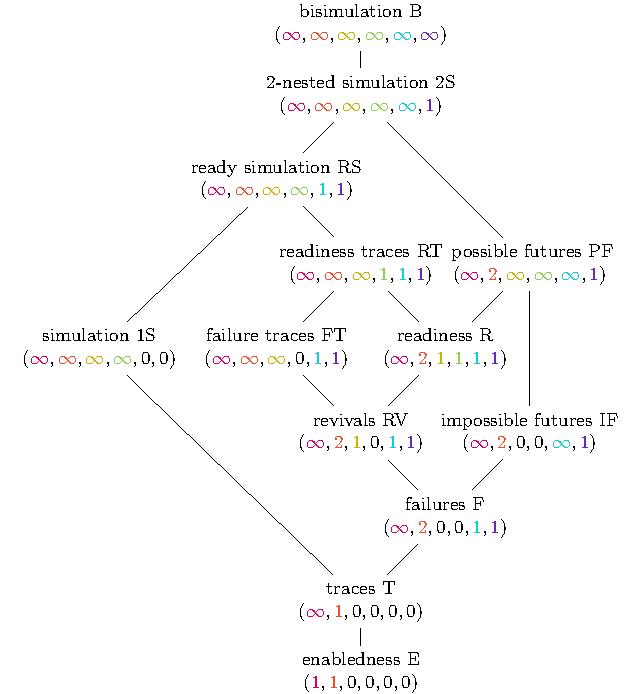
\includegraphics[height=200pt]{images/spectrum.pdf}
    \end{center}
    \tiny{Grafik: \textcite{bisping2023process}}
\end{frame}

%-------------------------------------------------------------------------------
\begin{frame}{Das Spektrum}
    \begin{center}
    Welche Kosten sind benötigt, um Prozesse 0 und 4 zu unterscheiden?

    $=$

    Welche Äquivalenzen gelten zwischen Prozessen 0 und 4?
    \vspace{1em}

    \exampleLTS
    \end{center}
\end{frame}

%-------------------------------------------------------------------------------
\begin{frame}{Energiespiele~\autocite{bisping2023process,brihaye2023multi}}
    \begin{columns}
    \begin{column}{0.4\textwidth}
        \begin{itemize}
            \item Reachability Game
                \uncover<2->{mit Kosten (Energien) auf den Kanten}
            \uncover<3->{\item Energien können mehrdimensional sein}
            \uncover<4->{\item Kosten erweitert durch $\mathtt{min}$-updates}
        \end{itemize}
    \end{column}
    \begin{column}{0.51\textwidth}
        \hspace{\fill}
        \begin{tikzpicture}
            [atk/.style={rectangle,draw,text=red,inner sep=2mm},
             def/.style={circle,draw,text=blue,inner sep=1mm},
             energy/.style={gray},
             ->,
             level distance=20mm,
             level 1/.style={sibling distance=30mm},
             level 2/.style={sibling distance=12mm}]
            \node[atk] (a0) {$a_0$}
                child {node[atk] (a1) {$a_1$}
                    child {node[def] (d0) {$d_0$} edge from parent node[left] {
                            \only<2>{$-1$}%
                            \only<3->{$-1, 0$}%
                    }}
                    child {node[def] (d1) {$d_1$} edge from parent node[right=0mm] {
                            \only<2>{$-2$}%
                            \only<3->{$0, -1$}%
                    }}
                    edge from parent node[left] {
                        \only<2>{$-1$}%
                        \only<3>{$0, 0, -1$}%
                        \only<4->{$0, 0, \mathtt{min}_{\{2, 3\}}$}%
                    }
                }
                child {node[def] (d2) {$d_2$}
                    child {node[def] (d3) {$d_3$} edge from parent node[left,near start] {
                        \only<2>{$-5$}%
                        \only<3->{$0, -1$}%
                    }}
                    child {node[atk] (a2) {$a_2$} edge from parent node[left,inner sep=0] {
                        \only<2->{$-1$}%
                    }}
                    % Don't create an edge here, instead draw both edges with bends below
                    child {node[atk] (a3) {$a_3$} edge from parent[draw=none]}
                    edge from parent node[right] {
                        \only<2>{$-2$}%
                        \only<3>{$-1, 0, 0$}%
                        \only<4->{$\mathtt{min}_{\{1, 2\}}, 0, 0$}%
                    }
                };
            \draw[->,bend right=18] (d2) to node[right] {\only<2->{$0$}} (a3);
            \draw[->,bend right=18] (a3) to node[right] {\only<2->{$-1$}} (d2);
            \uncover<5->{
                \node[energy,below=0 of d0] {$0, 0, 0$};
                \node[energy,below=0 of d1] {$0, 0, 0$};
                \node[energy,below=0 of d3] {$0, 0, 0$};
            }
            \uncover<6->{
                \node[energy,left=0 of a1,align=right] {$1, 0, 0$\\$0, 1, 0$};
            }
            \uncover<7->{
                \node[energy,left=0 of d2] {$\emptyset$};
                \node[energy,left=0 of a0,align=right] {$1, 0, 0$\\$0, 1, 1$};
            }
        \end{tikzpicture}
    \end{column}
    \end{columns}
\end{frame}

%-------------------------------------------------------------------------------
\begin{frame}{Energiemengen}
Wir suchen die Menge der Energien, mit denen der Angreifer das Spiel
gewinnt.

\begin{columns}
\begin{column}{0.7\textwidth}
    \begin{block}{Energien}
        $\mathbf{En} = {(\mathbb{N} \cup \{ \infty \})}^6$\\
        Oberhalb-Menge von $E \subseteq \mathbf{En}$:
        \[\upclosed E := \{e \in \mathbf{En} \mid \exists a \in E\,.\,e \geq a\}\]
        Minimale Energien~\autocite{bisping2023process}:
        \[\mathrm{Min} (E) :=
            \{e \in E \mid \nexists e' \in E\,.\,e' \leq e \wedge e' \ne e\}\]
    \end{block}
\end{column}
\end{columns}

\end{frame}

\section{GPU-Implementierung Energiespiele}

\subsection{Angriffspositionen}

%-------------------------------------------------------------------------------
\begin{frame}[t]{Angriffspositionen}
\[\mathrm{Min} \left( \bigcup_{g' \in \mathrm{Succ}(g)} \upclosed E'_{g'} \right) =
  \mathrm{Min} \left( \bigcup_{g' \in \mathrm{Succ}(g)}           E'_{g'} \right)\]
\vspace{1em}

\only<1>{
\begin{center}
\begin{tikzpicture}[scale=0.8]
    \draw[fill=green,opacity=0.2] (1, 2) rectangle (4, 4);
    \draw[radius=2pt,fill] (1, 2) circle;
    \draw[fill=green,opacity=0.2] (2, 0) rectangle (4, 4);
    \draw[radius=2pt,fill] (2, 0) circle;

    \draw[<->,thick] (0, 4.2) -- (0, 0) -- (4.2, 0);
    \draw (0, 0) grid (4, 4);
    \foreach \x in {1, 2, 3, 4} {
        \node[anchor=north] at (\x, 0) {\scriptsize\x};
        \node[anchor=east] at (0, \x) {\scriptsize\x};
    }
    \node[anchor=north east] at (0, 0) {\scriptsize 0};
\end{tikzpicture}
\end{center}
}

\only<2>{
\begin{center}
\begin{tikzpicture}
    \node[rectangle,draw] (start_node) {\large{$g$}};
    \node (successor1) [right=of start_node,label=above:Nachfolger] {$g_1$};

    % Energies of successors
    \node (energy1_1) [right=of successor1] {$e_{g_1,1}$};
    \node (energy1_2) [below] at (energy1_1.south) {$e_{g_1,2}$};
    \node (dots1) [below] at (energy1_2.south) {\rvdots};
    \node (energy2_1) [below] at (dots1.south) {$e_{g_2,1}$};
    \node (energy2_2) [below] at (energy2_1.south) {$e_{g_2,2}$};
    \node (dots2) [below] at (energy2_2.south) {\rvdots};

    \node (successor2) [left=of energy2_1] {$g_2$};
    \node (dots_successors) at (successor2 |- dots2) {\rvdots};

    % Updated energies
    \node (updated1_1) [right=of energy1_1] {$e_{g_1,1}'$};
    \node (updated1_2) [right=of energy1_2] {$e_{g_1,2}'$};
    \node (udots1) at (updated1_2 |- dots1) {\rvdots};
    \node (updated2_1) [right=of energy2_1] {$e_{g_2,1}'$};
    \node (updated2_2) [right=of energy2_2] {$e_{g_2,2}'$};
    \node (udots2) at (updated2_2 |- dots2) {\rvdots};

    % Minimized energies
    \node (minimal1) [right=14mm of udots1.north] {$e_1^*$};
    \node (minimal2) [below] at (minimal1.south) {$e_2^*$};
    \node (mdots) [below] at (minimal2.south) {\rvdots};

    \draw[->] (start_node.east) -- (successor1.west);
    \draw[->] (start_node.east) -- (successor2.west);
    \draw[->] (successor1) -- (energy1_1.west);
    \draw[->] (successor1) -- (energy1_2.west);
    \draw[->] (successor1) -- (energy1_2.west |- dots1);
    \draw[->] (successor2) -- (energy2_1.west);
    \draw[->] (successor2) -- (energy2_2.west);
    \draw[->] (successor2) -- (energy2_2.west |- dots2);

    \draw[->] (energy1_1) -- node (l_update) [above=3mm] {Update} (updated1_1);
    \draw[->] (energy1_2) -- (updated1_2);
    \draw[->] (energy1_2.east |- dots1) -- (updated1_2.west |- udots1);
    \draw[->] (energy2_1) -- (updated2_1);
    \draw[->] (energy2_2) -- (updated2_2);
    \draw[->] (energy2_2.east |- dots2) -- (updated2_2.west |- udots2);

    % Diagonal lines suggesting the reduction to minimal energies
    \draw[thick] (updated1_1.east |- udots2.south) -- (minimal1.west |- mdots.south);
    \draw[thick] (updated1_1.north east) -- (minimal1.north west);
    \node (l_minimize) [right=4mm of l_update] {Minimieren};
\end{tikzpicture}
\end{center}
}
\end{frame}

\subsection{Verteidigungspositionen}

%-------------------------------------------------------------------------------
\begin{frame}[t]{Verteidigungspositionen}
    \[\text{\textbf{Gesucht:}}\quad\mathrm{Min} \left(
        \bigcap_{g' \in \mathrm{Succ}(g)} \upclosed E'_{g'} \right)\]

    \only<1>{
    \begin{center}
    \vspace{1em}
    \begin{tikzpicture}[scale=0.8]
        \draw[fill=green,opacity=0.2] (0, 3) rectangle (4, 4);
        \draw[radius=2pt,fill] (0, 3) circle;
        \draw[fill=green,opacity=0.2] (1, 1) rectangle (4, 4);
        \draw[radius=2pt,fill] (1, 1) circle;
        \draw[fill=green,opacity=0.2] (3, 0) rectangle (4, 4);
        \draw[radius=2pt,fill] (3, 0) circle;

        % Intersection
        \draw[fill=blue,opacity=0.15] (1, 3) rectangle (4, 4);
        \draw[fill=blue,opacity=0.15] (3, 1) rectangle (4, 4);


        \draw[<->,thick] (0, 4.2) -- (0, 0) -- (4.2, 0);
        \draw (0, 0) grid (4, 4);
        \foreach \x in {1, 2, 3, 4} {
            \node[anchor=north] at (\x, 0) {\scriptsize\x};
            \node[anchor=east] at (0, \x) {\scriptsize\x};
        }
        \node[anchor=north east] at (0, 0) {\scriptsize 0};

        % Suprema
        \draw[fill] (1, 3) +(-0.08, -0.08) rectangle +(0.08, 0.08);
        \draw[fill] (3, 1) +(-0.08, -0.08) rectangle +(0.08, 0.08);
        \draw[fill,gray] (3, 3) +(-0.08, -0.08) rectangle +(0.08, 0.08);
    \end{tikzpicture}
    \end{center}
    }

    \only<2->{
    \textbf{Schnittmenge von zwei Energiemengen:}
    \[\mathrm{Min} (\upclosed E_1 \cap \upclosed E_2 ) =
      \mathrm{Min} (\{ \sup(e_1, e_2) \mid e_1 \in E_1,\ e_2 \in E_2 \})\]
    \pause
    }

    \only<3>{
    \textbf{Iterative Schnittmenge:}~\autocite{brihaye2023multi}
    \footnotesize
    \setlength{\algomargin}{3em}
    \begin{algorithm}[H]
        \DontPrintSemicolon
        \SetKwData{Intersection}{intersection}
        \SetKwData{New}{new\_energies}
        \SetKwData{Updated}{updated}
        \SetKwData{Energies}{energies}

        $\New = \Updated[g_1]$ for some $g_1 \in \mathrm{Succ}(g)$\;
        \For{$g' \in \mathrm{Succ}(g) \setminus \{g_1\}$}{
            $\New = \{\sup(e_1, e_2) \mid e_1 \in \New,\ e_2 \in \Updated[g']\}$\;
            $\New = \mathrm{Min} (\New)$\;
        }
    \end{algorithm}
    }
\end{frame}


\section{Vorstellung des Programms}

%-------------------------------------------------------------------------------
\begin{frame}{Demo}
    \begin{columns}
    \begin{column}{0.46\textwidth}
        \exampleLTS
    \end{column}
    \begin{column}{0.54\textwidth}
        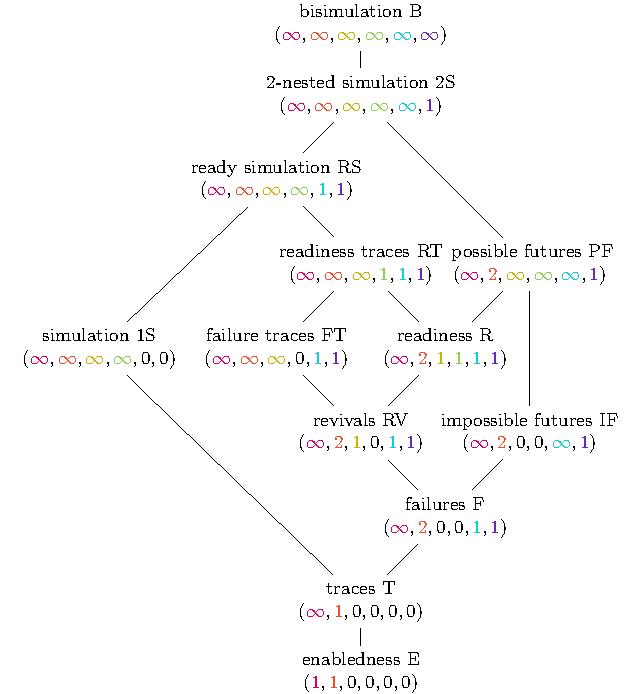
\includegraphics[width=\textwidth]{images/spectrum.pdf}
    \end{column}
    \end{columns}
\end{frame}

\subsection{Benchmarks}

%-------------------------------------------------------------------------------
\begin{frame}{VLTS Benchmarks}
\centering
\footnotesize
\begin{tabular}{@{}l
                r@{\hskip 6pt}r
                r@{\hskip 6pt}r
                S[table-format=3.2]@{\hskip 6pt}
                S[table-format=1.4]@{}
                S[table-format=3.4]@{}}
    \toprule
    &\multicolumn{2}{c}{Größe LTS}
    &\multicolumn{2}{c}{Größe Spielgraph}
    &\multicolumn{3}{c}{Laufzeit (s)} \\
    \cmidrule(lr){2-3} \cmidrule(lr){4-5} \cmidrule(l){6-8}
    LTS~\autocite{vlts}
    &$|\mathsf{Proc}|$ &$\sim_B$
    &$|G|$ &$|E|$
    &Scala~\autocite{bisping2023process} &{gpuequiv} &{Graph} \\
    \midrule

    \texttt{vasy\_0\_1}   &289    &9      &276        &844         &0.02   &0.0045 &0.0001  \\
    \texttt{vasy\_1\_4}   &1183   &28     &520        &1377        &0.02   &0.0053 &0.0002  \\
    \texttt{vasy\_5\_9}   &5486   &145    &1859       &3466        &0.06   &0.0051 &0.0007  \\
    \texttt{vasy\_8\_24}  &8879   &416    &59,761     &147,168     &2.15   &0.046  &0.026   \\
    \texttt{vasy\_8\_38}  &8921   &219    &7535       &21,643      &0.19   &0.0072 &0.003   \\
    \texttt{vasy\_10\_56} &10,849 &2112   &1,950,422  &6,064,252   &174.59 &4.047  &1.319   \\
    \texttt{vasy\_18\_73} &18,746 &4087   &76,010,111 &624,135,160 &{--}   &{--}   &108.872 \\
    \texttt{vasy\_25\_25} &25,217 &25,217 &0          &0           &0.33   &0.0017 &3.582   \\
    \texttt{cwi\_1\_2}    &1952   &1132   &8,504,998  &22,708,680  &384.13 &8.536  &5.197   \\
    \texttt{cwi\_3\_14}   &3996   &62     &11,094     &24,190      &0.3    &0.024  &0.003   \\
    \bottomrule
\end{tabular}
\end{frame}


\section*{Fazit}

%-------------------------------------------------------------------------------
\begin{frame}{Zusammengefasst}
    \begin{itemize}
        \item Idee: Schnellere Spektroskopie mithilfe von GPU
        \item Ergebnis: Rust library \texttt{gpuequiv} verfügbar auf
            \url{https://github.com/Gobbel2000/gpuequiv}
        \item Mittels WebGPU + WebAssembly auch im Browser
        \item Die Entscheidenden Berechnungen laufen parallel auf GPU
        \item Erzielt deutlich schnellere Laufzeiten
    \end{itemize}
\end{frame}

\section*{Quellen}

%-------------------------------------------------------------------------------
\begin{frame}{Quellen}
    \printbibliography
\end{frame}

\end{document}
